\documentclass{article}

\usepackage[utf8]{inputenc}
\usepackage[T1]{fontenc}
\usepackage[greek,english]{babel}
\usepackage{alphabeta}
\usepackage{amsmath}
\usepackage{amssymb}
\usepackage{graphicx}
\usepackage{subcaption}
\usepackage{epstopdf}
\usepackage[margin=1in, paperwidth=7.5in,paperheight=10.5in]{geometry}
\usepackage{hyperref}
\usepackage{paracol}

\newcommand\course{TΗΛ411}
\newcommand\courseName{Ψηφιακή Επεξεργασία Εικόνας}
\newcommand\semester{Χειμερινό 2021}
\newcommand\assignmentNumber{Assignment 8}
\newcommand\studentName{Μαυρογιώργης Δημήτρης}                           
\newcommand\studentNumber{2016030016}

\title{\underline{\textbf{\assignmentNumber}}} 
\author{\textsc{\textbf{Όνομα:}}  \studentName\\
		\textsc{\textbf{ΑΜ:}}  \studentNumber\\
		\course \ - \courseName\\ 
		\textsc{Πολυτεχνείο Κρήτης}
}
\date{\today}
\begin{document}
	\maketitle

\section*{Introduction}
	Ο σκοπός της 8ης εργαστηριακής άσκησης είναι να υπολογισουμε το μετασχηματισμο Fourier της εικόνας "cameran.tif", καθώς και ενός Gaussian φίλτρου. Επιπλέον, στόχος της συγκεριμένης άσκησης είναι να υπολογίσουμε τη συνέλιξη της εικόνας με το φίλτρο με τρεις διαφορετικούς τρόπους: 1) στο πεδίο του χρόνου, 2) στο πεδίο των συχνοτήτων με βάση το θεώρημα της συνέλιξης και 3) με το γινόμενο του πίνακα Toeplitz και της εικόνας.
	
\section*{Implementation-Results}
	 Αρχικά, μας ζητήθηκε να διαβάσουμε την εικόνα "camerama.tif" διαστάσεων 512x512 και την μετατρέψουμε σε διαστάσεις 30x30. Για το σκοπό αυτό χρησιμοποιήθηκε η συνάρτηση imresize με τα default της ορίσματα. 
	 
	\begin{figure}[h!]
		\centering
		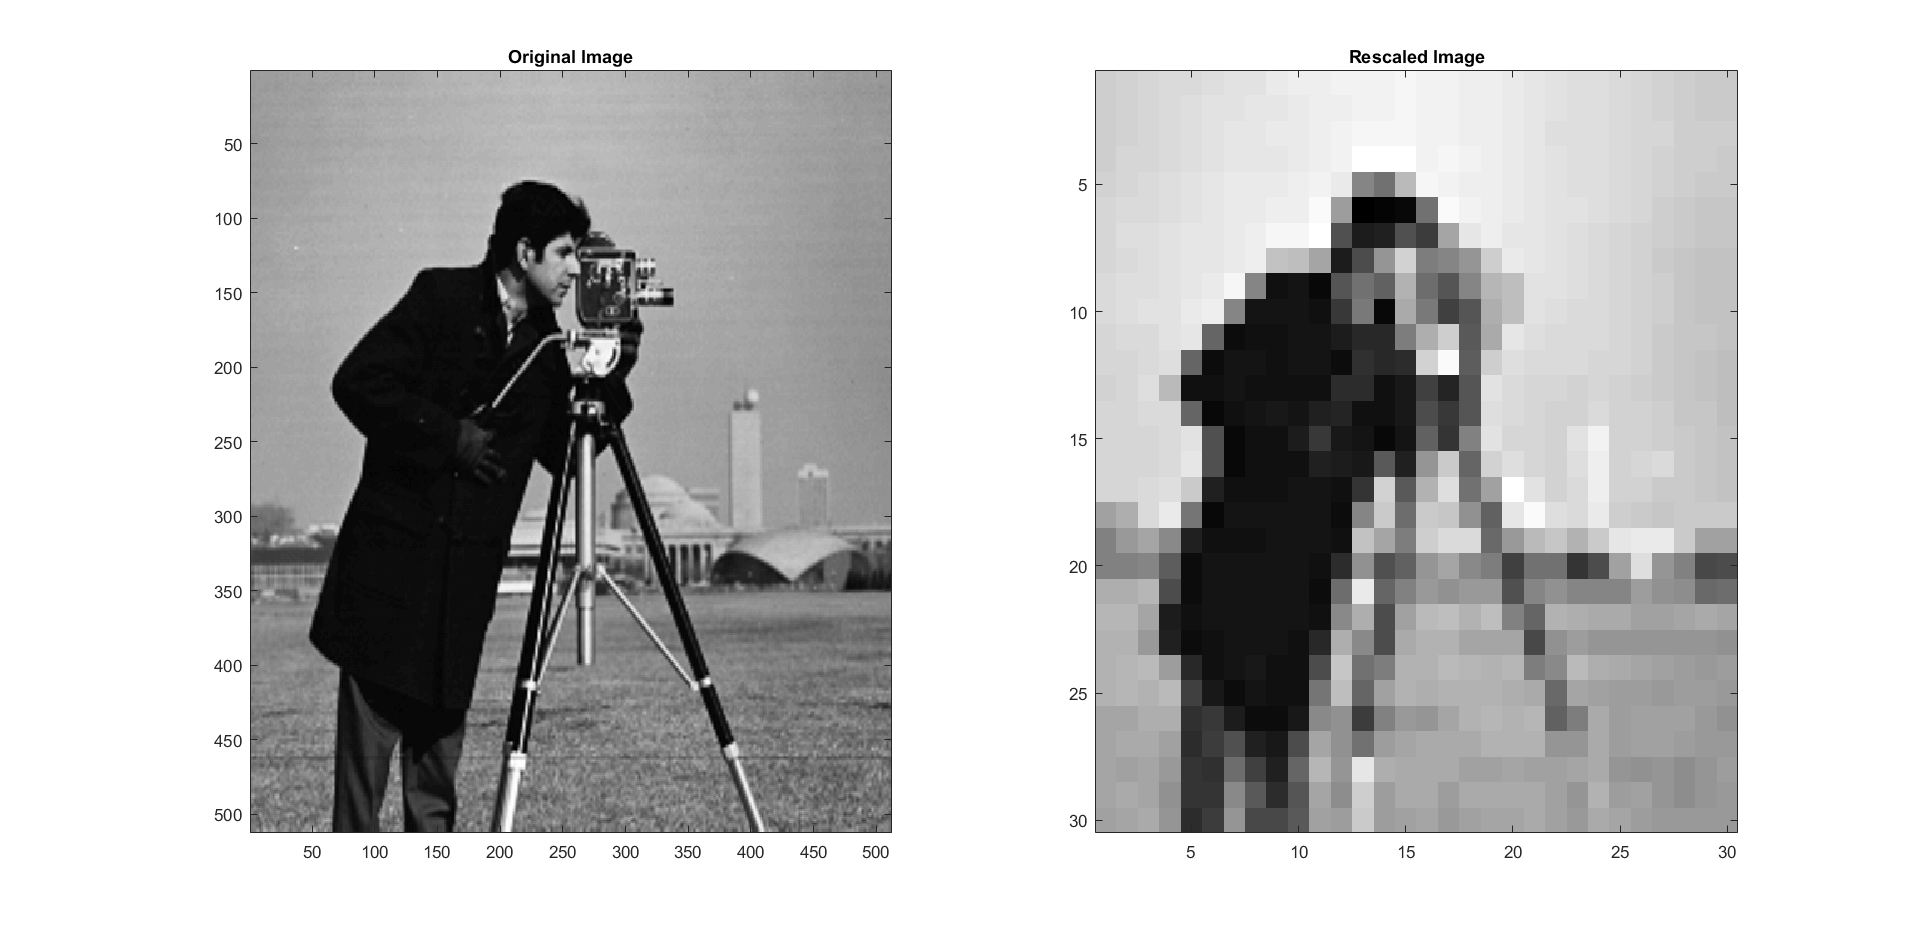
\includegraphics[ width=\linewidth]{./output_images/img_berfore_fft.png}
	\end{figure}

	\noindent
	Στη συνέχεια, μας ζητήθηκε να υπολογίσουμε το μετασχηματισμό Fourier της εικόνας διαστάσεων 30x30. Γι'αυτό το σκοπό χρησιμοποιήθηκε η συνάρτηση fft2 και fftshift. Παρακάτω απεικονίζονται σε κανονική και λογαριθμική κλίμακα τα αποτελέσματα του μέτρου του μετασχηματισμού Fourier, καθώς και του φάσματος της εικόνας, δηλαδή το τετράγωνο του μέτρου του μετασχηματισμού Fourier μετά τη χρήση της συνάρτησης fft2 και fftshift.

	\pagebreak
	\begin{figure}[h!]
		\centering
		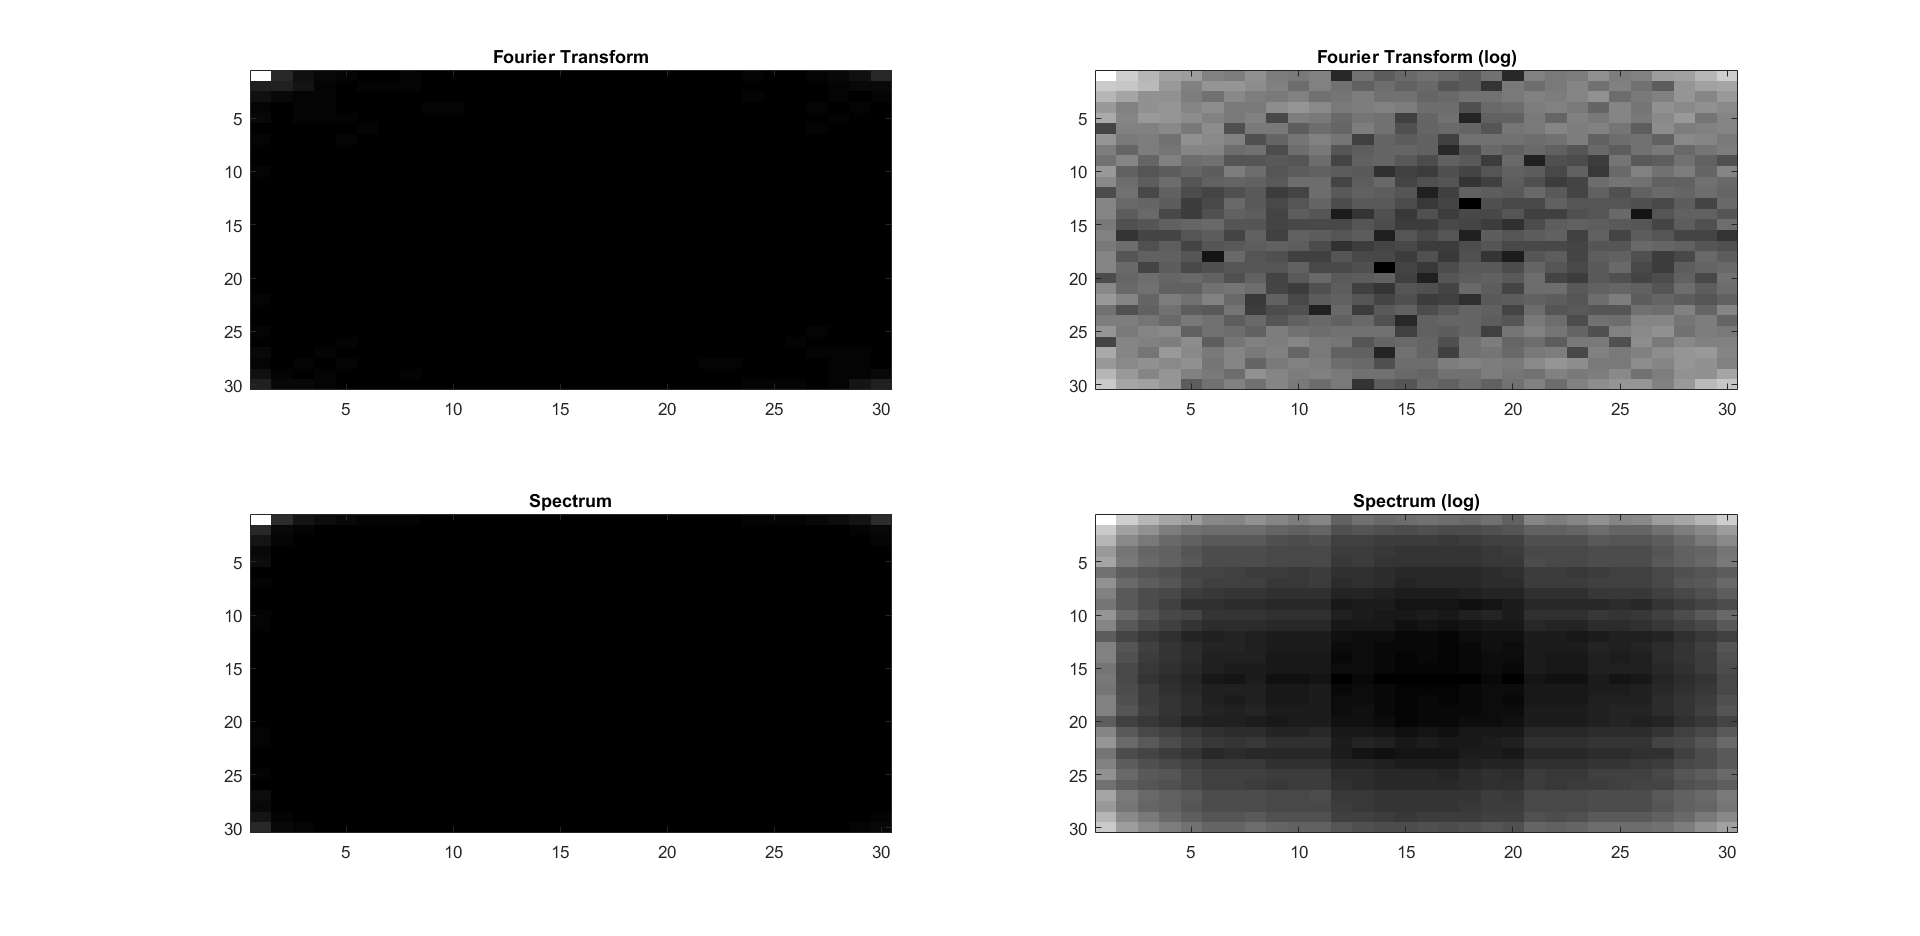
\includegraphics[ width=\linewidth]{./output_images/img_after_fft.png}
	\end{figure}

	\begin{figure}[h!]
		\centering
		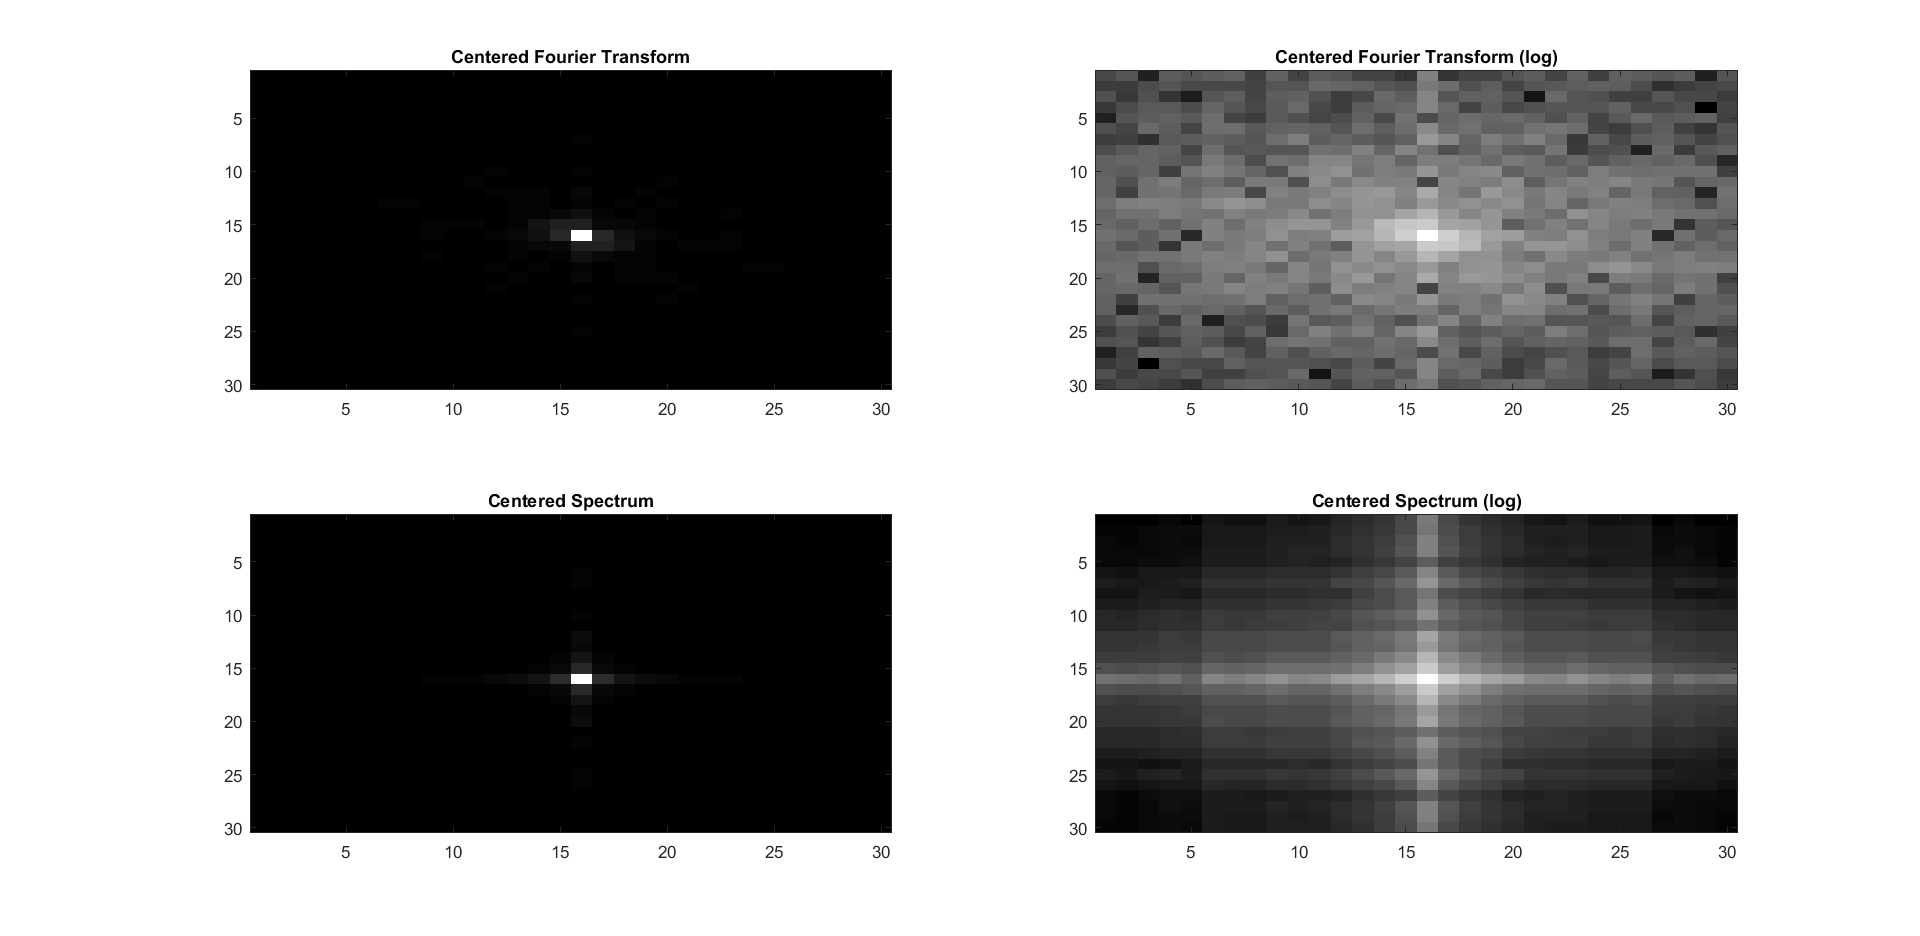
\includegraphics[ width=\linewidth]{./output_images/img_after_fft_shift.png}
	\end{figure}

	\noindent
	Μετά τον υπολογισμό και την απεικόνιση του μέτρου του μετασχηματισμού Forrier και του φάσματος της εικόνας, μας ζητήθηκε να κατασκευάσουμε ένα 2D Gaussian φίλτρο 9x9 με τη βοήθεια της συνάρτησης meshgrip. Έπειτα, υπολογίστηκε και ο μετασχηματισμός Fourier του φίλτρου. Με τη βοήθεια της συνάρτησης mesh απεικονίστηκε το Gaussian φίλτρο τόσο στο χρόνο, όσο και στη συχνότητα. Aυτό που παρατηρούμε είναι ότι το φίλτρο στις συχνότητες διατηρεί το καμπανοειδές σχήμα που έχει στο χρόνο. Η μοναδική διαφορά είναι ότι στο χρόνο το σχήμα του φίλτρου είναι πιο λεπτό και μυτερό, ενώ στη συχνότητα είναι αρκετά πιο φαρδύ και ομαλό.	
	
	\pagebreak
	\begin{figure}[h!]
		\centering
		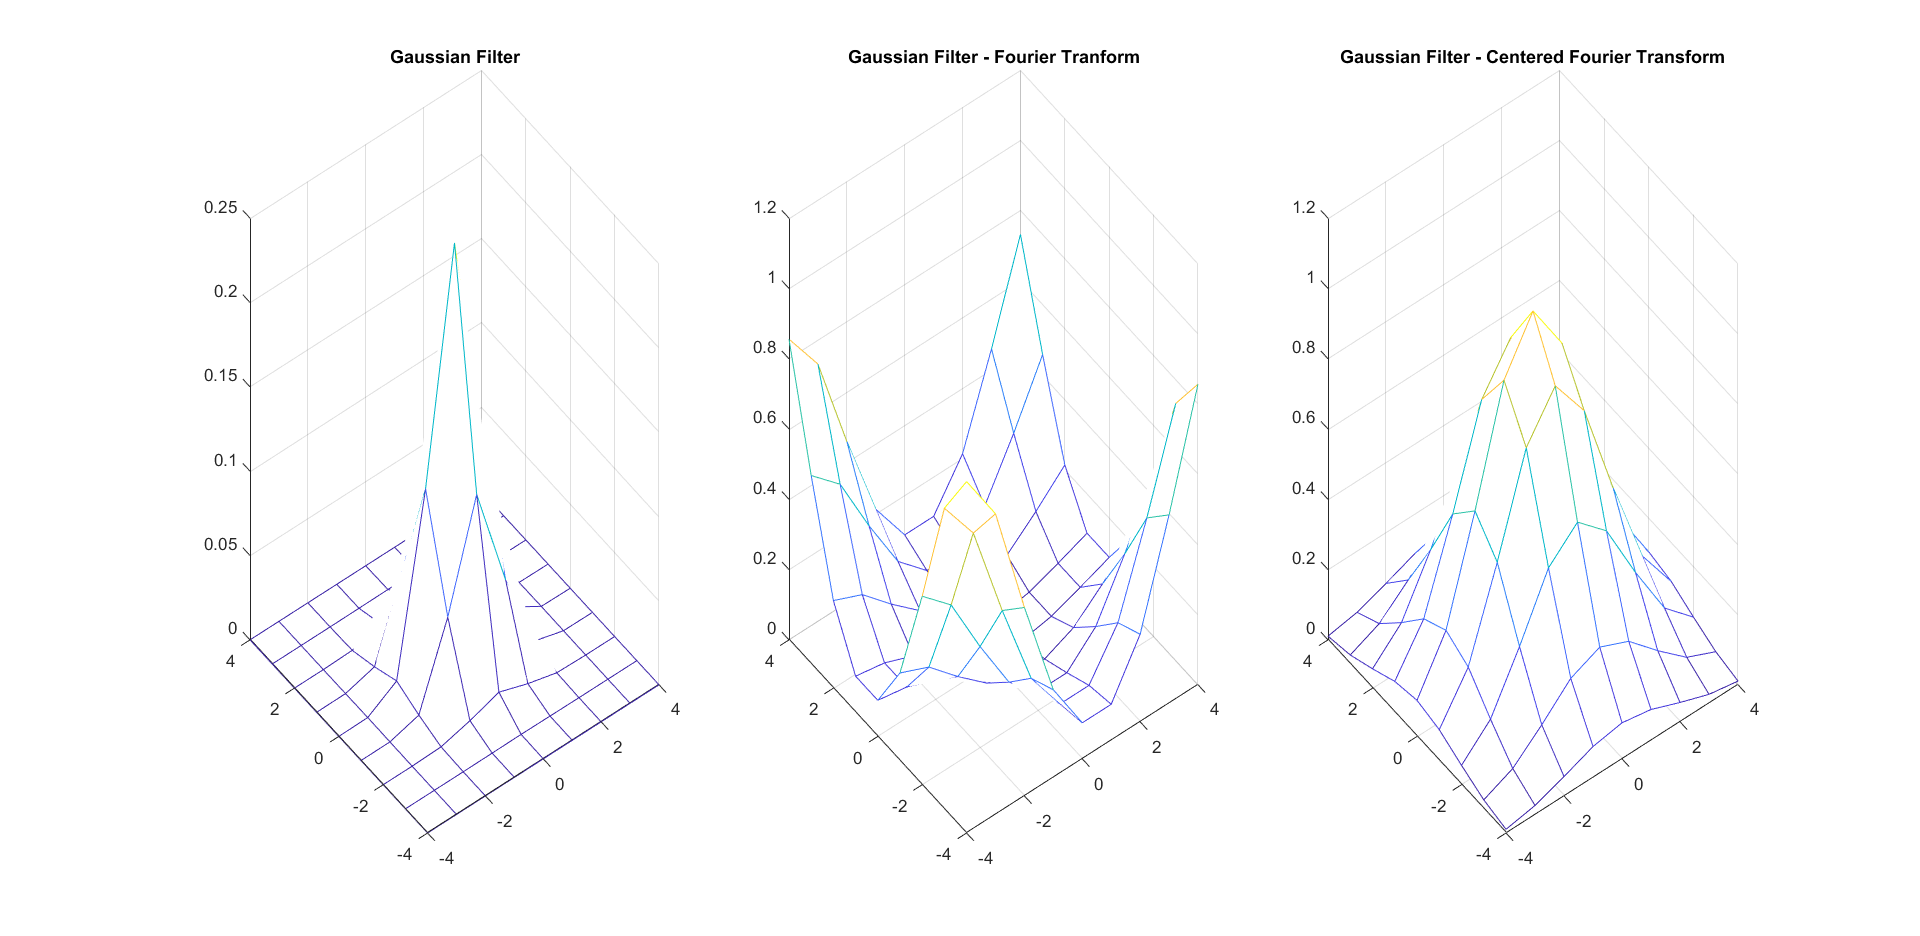
\includegraphics[ width=\linewidth]{./output_images/gaussian_filter.png}
	\end{figure}
	
	\noindent
	Στο τελευταίο μέρος της άσκησης, έπρεπε να υπολογίσουμε τη συνέλιξη του παραπάνω φίλτρου με την εικόνα cameraman διαστάσεων 30x30 με τρεις διαφορετικούς τρόπους.\\
	
	\begin{figure}[h!]
		\centering
		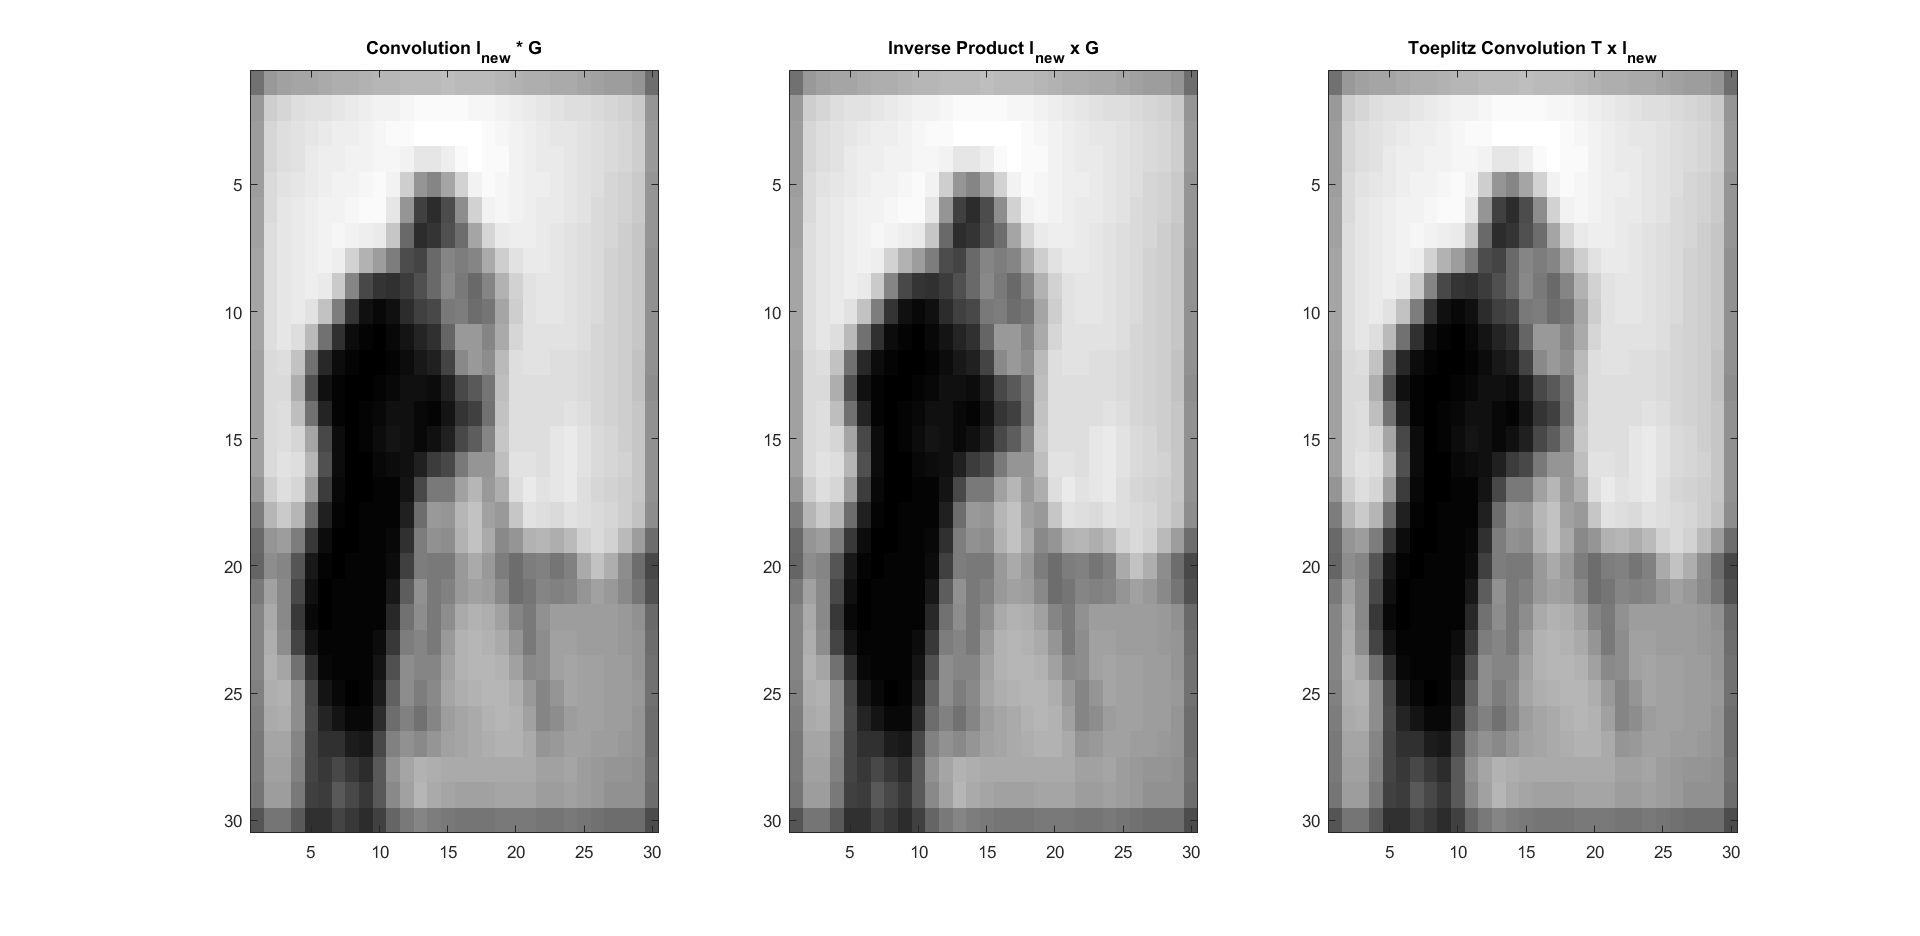
\includegraphics[ width=\linewidth]{./output_images/conv2_convTheorem_toeplitz.png}
	\end{figure}

	\noindent
	Στην πρώτη μέθοδο για τον υπολογισμό της συνέλιξης στο πεδίο του χρόνο χρησιμοποιήθηκε η συνάρτηση conv2 με ορίσματα την εικόνα, το φίλτρο και παράμετρο 'same', για να παραμείνει εικόνα σε διαστάσεις 30x30 και όχι (30+9-1)x(30+9-1)=38x38 που θα ήταν με το zero padding.\\
	
	\noindent
	Η δεύτερη μέθοδος υπολογισμού της συνέλιξης είναι μεσω του πεδίου των συχνοτήτων και το θεώρημα συνέλιξης, το οποίο αναφέρει ότι στη συχνότητα η συνέλιξη υπολογίζεται ως το γινόμενο του μετασχηματισμού Fourier της εικόνας και του μετασχηματισμού Fourier του φίλτρου. Για τον υπολογισμό του γινομένου, έπρεπε πρώτα να κάνουμε zero padding έτσι, ώστε η εικόνα και το φίλτρο να είναι και οι δύο διαστάσεων 38x38. Aυτό έγινε με τη συνάρτηση fft2, η οποία κάνει zero padding, αν εκτος επό την εικόνα περάσουμε σαν ορίσματα και τις τελικές διαστάσεις της εικόνας. Τέλος, μετά τον υπολογισμό του γινομένου χρησιμοποιήθηκε η συνάρτηση ifft2 για να υπολογίσουμε τον αντίστροφο μετασχηματισμό Fourier.
	
	\pagebreak  
	\noindent
	Στην τρίτη και τελευταία μέθοδο, έπρεπε να υπολογίσουμε την συνέλιξη μέσω του γινομένου του πίνακα toeplitz και της εικόνας σε μορφή vector. Οι διαστάσεις της τελικής εικόνας είναι 38x38, οπότε σε μορφή vector θα είναι 1444x1. Επίσης, η αρχική εικόνα είναι 30x30. Οπότε σε μορφή vector θα είναι 900x1. Συνεπώς, ο πίνακας toeplitz πρέπει να έχει διαστάσεις 1444x900 για να μπορέσει να γίνει το γινόμενο. \\
	
	\noindent
	Όσον αφορά τη διαδικασία υπολογισμού του πίνακα toeplitz, έγιναν τα εξής βήματα:
	\noindent
	\begin{itemize}
		\item[1)] Ζero padding στο Gaussian φίλτρο έτσι, ώστε να γίνει διαστάσεων 38x38 και να έχει μη μηδενικά στοιχεία στο κάτω αριστερά μερος του.
		\item[2)] Για κάθε γραμμή του φίλτρου υπολογίστηκαν οι 38 υποπίνακες toeplitz διαστάσεων 38x30.
		\item[3)] Mε τη βοήθεια της συνάρτηση cat ένώθηκαν και οι 38 πίνακες ετσι, ώστε να υπολογιστεί η πρώτη block στήλη του πίνακα tοeplitz.
		\item[4)] Mε τη βοήθεια της συνάρτηση circshift έγιναν shift οι block πίνακες προς τα κάτω και κυκλικά, για να υπολογιστούν και οι υπόλοιπες στήλες του πίνακα tοeplitz.
		\item[5)] Mε τη συνάρτηση cat ένώθηκαν και οι 30 στήλες του προηγούμενου βήματος ετσι, ώστε να υπολογιστεί ο τελικός πίνακας toeplitz.
	\end{itemize}

	\noindent
	Στη συνέχεια, χρησιμοποιήθηκε η συνάρτηση flip για να διαβάσουμε τις τιμές από την τελευταια γραμμή προς την αρχική και σε συνδυασμό με ένα βρόγχο επανάληψης μετατράπηκε η εικόνα σε vector προκειμένου να γίνει ο πολλαπλασιασμός με τον πίνακα. Τέλος, αφού έγινε ο πολλαπλασιασμός, χρησιμοποιήθηκαν οι συνάρτησεις reshape και flip, για να επαναφέρουμε την εικόνα από vector σε πίνακα.\\
	
	\noindent
	Στο τελεταίο κομματι της άσκησης, έπρεπε να γίνει η σύσκριση των τριών μεθόδων για συνέλιξης της εικόνας με το Gaussian φίλτρο. Με βάση τις παραπάνω εικόνες, παρατηρούμε ότι είναι όλες ίδιες μεταξύ τους. Αυτό βεβαιώνεται με από το δείκτη MSE, ο οποίος ανάμεσα μέθοδο 1 και 2 είναι $1.4490 \cdot 10^{-27}$, μεταξύ των μεθόδων 1 και 3 είναι $3.6431 \cdot 10^{-27}$ και τέλος μεταξύ της 2 και 3 είναι $3.2437 \cdot 10^{-27}$.
	 	
\end{document}
